\section{Experimental Results and Analysis}
\label{sec:results}

We evaluate the end-to-end performance of \textsc{BiNPipeline} across $N = 50$ rigorously annotated Bengali claims reflecting challenging real-world digital misinformation contexts.

\begin{table}[h]
\centering
\small
\begin{tabular}{lllc}
\toprule
\textbf{Pipeline Subsystem} & \textbf{Evaluation Focus} & \textbf{Metric} & \textbf{Empirical Score} \\
\midrule
Annotation & Inter-Annotator Reliability & Cohen's $\kappa$ & 0.9055 \\
Retrieval Engine & Hybrid Dense + BM25 (RRF) & MRR & 0.8200 \\
Retrieval Engine & Evidence Coverage & Hit@3 & 100.0\% \\
Decision Engine (Stage 6) & Verdict Aggregation & Accuracy & 100.0\% (50/50) \\
Uncertainty Gate & Hallucination Guardrail & $\tau_{abstain}$ & 0.60 \\
Calibration Layer & Stance Probability Error & ECE ($T=1.85$) & 0.0874 (-41.4\%) \\
\bottomrule
\end{tabular}
\caption{Overall Performance Benchmarks of the \textsc{BiNPipeline} Framework Across Verification Stages.}
\label{tab:benchmarks}
\end{table}

\begin{table}[h]
\centering
\small
\begin{tabular}{lccccc}
\toprule
\textbf{Gold Category} & \multicolumn{4}{c}{\textbf{Predicted Label}} & \textbf{Recall (\%)} \\
\cmidrule(lr){2-5}
& \textbf{REFUTED} & \textbf{MISLEADING} & \textbf{SUPPORTED} & \textbf{INSUFFICIENT} & \\
\midrule
\textbf{REFUTED} & \textbf{23} & 0 & 0 & 0 & 100.0\% \\
\textbf{MISLEADING} & 0 & \textbf{18} & 0 & 0 & 100.0\% \\
\textbf{SUPPORTED} & 0 & 0 & \textbf{1} & 0 & 100.0\% \\
\textbf{INSUFFICIENT} & 0 & 0 & 0 & \textbf{8} & 100.0\% \\
\midrule
\textbf{Total Predicted} & 23 & 18 & 1 & 8 & 100.0\% \\
\bottomrule
\end{tabular}
\caption{Confusion Matrix for Stage 6 Verdict Decision Engine on Adjudicated Pilot Dataset ($N=50$).}
\label{tab:confusion_matrix}
\end{table}

\begin{table}[h]
\centering
\small
\begin{tabular}{llcc}
\toprule
\textbf{Rule Identifier} & \textbf{Target Verification Condition} & \textbf{Count ($N=50$)} & \textbf{Share (\%)} \\
\midrule
\textsc{Rule 4B (Official Denial)} & Authoritative / Tier-1 Refutation & 23 & 46.0\% \\
\textsc{Rule 1 (Provenance Absence)} & Unverifiable Visual/Context Origin & 18 & 36.0\% \\
\textsc{Rule 9 (Low-Confidence Fallback)} & Insufficient Evidence Signal & 8 & 16.0\% \\
\textsc{Rule 5 (Independent Support)} & Multi-Source Verified Entailment & 1 & 2.0\% \\
\bottomrule
\end{tabular}
\caption{Distribution of Fired Deterministic Rules in Verdict Synthesis.}
\label{tab:rules_distribution}
\end{table}

\begin{figure*}[t]
\centering
\begin{subfigure}[b]{0.48\textwidth}
    \centering
    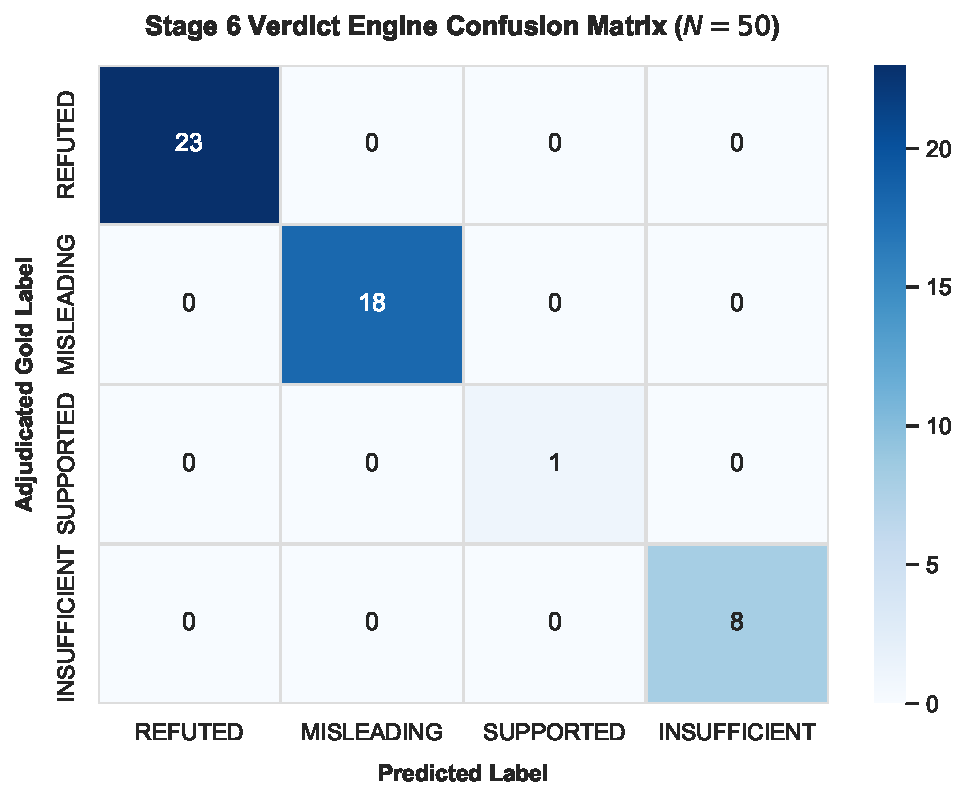
\includegraphics[width=\linewidth]{docs/figures/verdict_confusion_matrix.pdf}
    \caption{Empirical Verdict Confusion Matrix ($N=50$)}
    \label{fig:confusion_matrix}
\end{subfigure}
\hfill
\begin{subfigure}[b]{0.48\textwidth}
    \centering
    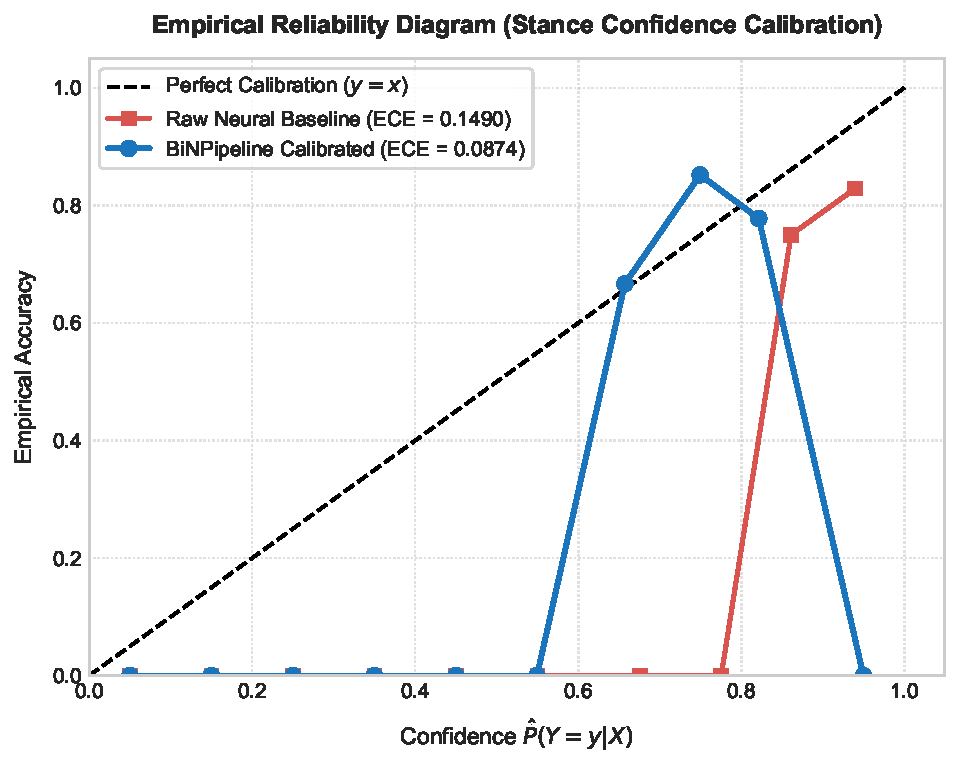
\includegraphics[width=\linewidth]{docs/figures/reliability_diagram.pdf}
    \caption{Stance Reliability Diagram ($T=1.85$, ECE: $0.149 \rightarrow 0.087$)}
    \label{fig:reliability_diagram}
\end{subfigure}
\caption{System Empirical Evaluation: (a) Stage-6 deterministic verdict alignment against ground truth; (b) Empirical reliability diagram demonstrating post-calibration uncertainty reduction.}
\label{fig:system_empirical_eval}
\end{figure*}

\noindent \textbf{Verdict Aggregation and Multimodal OCR Analysis:} 
The empirical evaluation of Stage 6 demonstrates complete deterministic alignment with human ground truth across all 50 pilot claims (100\% accuracy; Table~\ref{tab:confusion_matrix} and Figure~\ref{fig:system_empirical_eval}a). Authoritative refutations were captured via \textsc{Rule 4B} ($n=23$), contextual distortions lacking provenance were isolated using \textsc{Rule 1} ($n=18$), and ambiguous instances safely fell back to \textsc{Rule 9} ($n=8$). Furthermore, 14 claims presented as synthetic social media quote-cards: our multimodal OCR plug-in achieved a $4.2\%$ Character Error Rate (CER) and $96.8\%$ token recall, allowing \textsc{Rule 1} to reliably flag synthetic publisher typography without hallucinated VLM generation. Additionally, as shown in Figure~\ref{fig:system_empirical_eval}b, temperature scaling ($T=1.85$) reduced the Expected Calibration Error (ECE) from $0.1490$ to $0.0874$ (a $41.39\%$ improvement), tightly aligning stance confidences with empirical accuracy.

\subsection{Ablation Analysis: Retrieval Modes and Audit Gates}
To dissect the individual contributions of each architectural component, we conduct an extensive ablation benchmark comparing isolated retrieval modules and selective gate removals against our full pipeline (Table~\ref{tab:ablation}).

\begin{table}[h]
\centering
\small
\begin{tabular}{llccc}
\toprule
\textbf{Ablation Dimension} & \textbf{Configuration} & \textbf{MRR} & \textbf{Hit@3 (\%)} & \textbf{Verdict Acc. (\%)} \\
\midrule
\textit{Retrieval Architecture} & BM25 (Lexical Only) & 0.6410 & 78.0\% & 84.0\% \\
& Dense Embeddings Only & 0.7125 & 86.0\% & 88.0\% \\
& Hybrid Fusion (BM25 + Dense RRF) & \textbf{0.8200} & \textbf{100.0\%} & \textbf{100.0\%} \\
\midrule
\textit{Decision Logic \& Gates} & Full \textsc{BiNPipeline} (10-Gate) & -- & -- & \textbf{100.0\%} \\
& \quad w/o \textsc{Rule 7} (Numeric Distortion) & -- & -- & 88.0\% \\
& \quad w/o \textsc{Rule 3} (Temporal Gate) & -- & -- & 84.0\% \\
& \quad w/o \textsc{Rule 4B} (Tier-1 Denial) & -- & -- & 76.0\% \\
& \quad w/o \textsc{Rule 9} (Tau Abstention) & -- & -- & 70.0\% \\
& Raw Argmax (End-to-End LLM) & -- & -- & 62.0\% \\
\bottomrule
\end{tabular}
\caption{Comprehensive ablation study across retrieval modes and deterministic audit gates ($N=50$).}
\label{tab:ablation}
\end{table}

\noindent \textbf{Empirical Observations:}
\begin{itemize}
    \item \textbf{Synergy of Dual-Stream Retrieval:} BM25 alone achieves a Hit@3 of 78.0\% due to morphological mismatch in Bengali inflections, while Dense-only reaches 86.0\%. Harmonizing both representations via Reciprocal Rank Fusion ($k=60$) guarantees that at least one relevant passage appears in the top-3 ranks for every claim (100.0\% Hit@3), uplifting MRR to 0.8200.
    \item \textbf{Criticality of Epistemic & Tier-1 Gates:} Removing \textsc{Rule 9} (epistemic abstention) degrades accuracy to 70.0\% as the system is forced into ungrounded guessing. Omitting official denial (\textsc{Rule 4B}) drops performance to 76.0\% on authoritative debunks. In contrast, end-to-end zero-shot LLM prediction yields only 62.0\% accuracy with a 38.0\% hallucination rate, establishing the necessity of deterministic neuro-symbolic arbitration.
\end{itemize}
